%% A Lakehouse on Google Drive
%%
%% PVLDB experience-track style. Built with `make` in this directory; the
%% acmart class is vendored under cls/ because it is not in every distro's
%% base texlive install (see README.md).
%%
%% STATUS: sections 2 and 3 are drafted. Sections 1, 4-7 are outlined stubs
%% carrying the plan's per-section notes as comments. Every numeral in a
%% drafted section is traceable to docs/benchmark.md or to a named test; a
%% number that is not yet measured is written as \todonum{} so it cannot be
%% mistaken for a result.

\documentclass[sigconf, nonacm]{acmart}

\usepackage{booktabs}
\usepackage{balance}
\usepackage{xcolor}
\usepackage{pgfplots}
\pgfplotsset{compat=1.18}

\settopmatter{printacmref=false}
\renewcommand\footnotetextcopyrightpermission[1]{}
\pagestyle{plain}

%% acmart draws a ZapfDingbats glyph in the title block. That font ships in
%% texlive-fontsrecommended, which is not installed everywhere, and its
%% absence is a hard stop rather than a warning. The glyph is decorative, so
%% we drop it rather than make the build depend on an optional package.
\AtBeginDocument{\providecommand{\ding}[1]{}\renewcommand{\ding}[1]{}}

%% An unmeasured number. Deliberately loud: the paper must not ship with one.
\newcommand{\todonum}[1]{\textcolor{red}{\textbf{[?~#1]}}}
%% A cross-reference to the experiment register in Section 4.
\newcommand{\expref}[1]{\textsf{E-#1}}

\begin{document}

\title{A Lakehouse on Google Drive}
\subtitle{Building a DuckDB Filesystem on Storage That Is Not an Object Store}

\author{Joachim Rosskopf}
\affiliation{%
  \institution{DataZoo GmbH}
  \country{Germany}
}
\email{jr@data-zoo.de}

\begin{abstract}
We present \texttt{duckdb-gdrive}, a DuckDB extension that registers a
\texttt{gdrive://} filesystem over Google Drive, allowing
\texttt{read\_parquet}, \texttt{glob}, \texttt{COPY} and the DuckLake
lakehouse format to address Drive files with no download step. Drive is not an
object store: it has no path addressing, permits two files to share a name in
one folder, provides no atomic replace and no way to pin a read to a revision,
and charges 1.2--2.1\,s for a ranged read whose cost is nearly independent of
its length. We show how these properties invert the usual design --- fetching
\emph{more} data in \emph{fewer} requests is faster --- and describe the
identity-scoped caches, the revision-keyed shared block cache, and the
idempotency rules that follow. We then compare, guarantee by guarantee, what
S3 and GCS provide against what Drive provides, and give a verification
protocol for each claim rather than asserting it. A cold columnar scan of an
87\,MB Parquet file costs 3.05$\times$ the same file on GCS at our defaults and
2.02$\times$ when tuned, against roughly 30$\times$ for a local file. Our central
finding is that a lakehouse format is a better fit for Drive than a plain
filesystem is, precisely because it never mutates a file --- and that this
immutability is not merely a safety property but an exploitable one. Removing
metadata round trips the system already had the answers to cuts a 150-file read
by 47\%.
\end{abstract}

\maketitle

%% =====================================================================
\section{Introduction}
%% OUTLINE (plan sec. 1). Four run-in-headed paragraphs plus contributions:
%%   - Where analytical data actually lives.
%%   - Drive is not an object store.
%%   - Our approach: a VFS subclass, and the inheritance claim.
%%   - Why guarantees are the interesting part.
%% Contributions: (i) design + measured justification; (ii) guarantee-by-
%% guarantee comparison against S3/GCS with a verification protocol each;
%% (iii) DuckLake end-to-end evaluation; (iv) negative results.
%% Drafted last, after Sections 2-5 fix the terminology and the numbers.

\textbf{Where the data actually is.}
A great deal of the tabular data an organisation analyses does not live in an
object store. It lives in Google Drive, because that is where the people who
produced it put it: exports from operational systems, hand-maintained
reference tables, monthly extracts, the spreadsheet that is the system of
record for one department. The standard way to query it is to download it
first --- by hand, or with a synchronisation client, or through a scheduled
copy into a warehouse. Each of those makes a second copy that is immediately
stale, and each adds a component to provision and watch.

\textbf{Drive is not an object store.}
The obvious fix is to treat Drive as remote storage and read it in place, the
way DuckDB's \texttt{httpfs} reads S3. That fails on three structural
differences. Drive has no path addressing, so a path costs one listing request
per segment. It permits duplicate names, so a path is not a key. And its
ranged reads cost 1.2--2.1\,s almost regardless of how many bytes they request,
which makes Parquet's fine-grained ranged access the worst request pattern.
Section~\ref{sec:background} measures all three.

\textbf{Our approach.}
\texttt{duckdb-gdrive} implements a DuckDB \texttt{FileSystem} for the
\texttt{gdrive://} scheme. Because DuckDB dispatches all file access through
its virtual filesystem, everything layered on top inherits the scheme:
\texttt{read\_parquet}, \texttt{read\_csv}, \texttt{glob}, \texttt{COPY}, and
the DuckLake lakehouse format. The design work is almost entirely in the
caches and retry rules. Section~\ref{sec:design} describes both, and attaches
each choice to the measurement that produced it, including the ones we got
wrong first.

\textbf{Why the guarantees are the interesting part.}
A lakehouse format is a contract with its storage layer. DuckLake, Iceberg and
Delta Lake were designed against object-store semantics: unique keys, atomic
single-object writes, strongly consistent listing. Running one on Drive is
therefore a correctness question before it is a performance question. Passing
tests do not answer it. Section~\ref{sec:guarantees} sets the contracts side
by side and attaches a verification experiment to every row, including rows
where Drive's documentation does not say and we have not yet measured it.

\textbf{Contributions.}
\begin{itemize}
\item The design of a filesystem for storage with a high, size-independent
  per-request cost, and the measurements that justify each mechanism
  (Sections~\ref{sec:background}--\ref{sec:design}).
\item A guarantee-by-guarantee comparison of Google Drive against S3 and GCS,
  with an experiment attached to each claim (Section~\ref{sec:guarantees}).
\item An evaluation covering single-file scans, block-size sensitivity, and
  DuckLake end to end over three storage backends
  (Section~\ref{sec:eval}).
\item A set of negative results --- a read-ahead buffer that an external review
  recommended and that measurement refuted, a block size that was noise, and a
  per-request latency figure that was never measured and was wrong by up to
  14$\times$ --- reported because each was the natural thing to believe.
\end{itemize}

%% =====================================================================
\section{Background: Drive Is Not an Object Store}
\label{sec:background}

Google Drive exposes a REST API over a hierarchical, user-facing document
store. It is tempting to read that API as an object store with unusual
spelling. It is not one, and four differences matter enough that every design
decision in Section~\ref{sec:design} follows from them.

\textbf{There is no path addressing.}
Drive addresses content by opaque file id. There is no endpoint that accepts
\texttt{a/b/c.parquet}. Resolving that path means listing the children of the
root to find \texttt{a}, listing \texttt{a} to find \texttt{b}, and listing
\texttt{b} to find \texttt{c.parquet} --- one \texttt{files.list} per segment,
each costing a network round trip. A filesystem interface, meanwhile, is
defined entirely in terms of paths. Bridging that gap cheaply is the largest source
of avoidable work in the system, and it was the risk we thought most likely to
sink the project before we wrote code.

\textbf{A path is not a key.}
Drive permits two files with the same name in the same folder. This is not a
pathological case that a careful user avoids; it is what the web interface
produces when the same file is uploaded twice. The consequence for a
filesystem is severe: \texttt{gdrive://reports/q3.parquet} may denote two
distinct byte streams, and any implementation that silently returns one of
them makes query results depend on Drive's internal result ordering. We treat
ambiguity as an error (Section~\ref{sec:resolution}), which is the only
choice that is not quietly wrong.

\textbf{Cost is a function of request shape, not request size.}
Table~\ref{tab:latency} gives per-request latency by endpoint and shape,
measured over a warm keep-alive connection so that no TLS handshake is
included. Two rows carry the whole argument of this paper. A 1\,KiB ranged
read of an 87\,MB object costs 1348\,ms at the median; a 1\,MiB ranged read of
the same object costs 1375\,ms. Asking for a thousand times more data is free.
Yet a whole read of a \emph{small} file costs 569\,ms, less than half of
either. The unit of cost is therefore not ``a Drive round trip'' --- a figure
that does not exist --- but ``a ranged read of a large object'', the request a
Parquet scan is made of. A total does not say whether the cost is addressable.
Section~\ref{sec:breakdown} decomposes each request kind into connection
setup, server time and transfer, and places the resulting spans on a
wall-clock timeline. That decomposition, not the totals here, tells us which
part of the floor is ours to remove and which belongs to Google.

\begin{table}[t]
\caption{Per-request latency by endpoint and request shape. Warm keep-alive
session, service-account identity, p50 of 5--10 samples. Ranged rows read
from one 87\,MB Parquet object. Measured by \texttt{make latency}.}
\label{tab:latency}
\small
\begin{tabular}{lrrr}
\toprule
Request & min & \textbf{p50} & p90 \\
\midrule
\texttt{files.list} (one path segment)      & 291\,ms  & \textbf{330\,ms}  & 486\,ms \\
\texttt{files.get} (metadata)               & 263\,ms  & \textbf{293\,ms}  & 326\,ms \\
\texttt{alt=media}, whole 100-byte file     & 509\,ms  & \textbf{569\,ms}  & 730\,ms \\
\texttt{alt=media}, 1\,KiB range            & 1223\,ms & \textbf{1348\,ms} & 2491\,ms \\
\texttt{alt=media}, 1\,MiB range            & 1297\,ms & \textbf{1375\,ms} & 2342\,ms \\
\texttt{alt=media}, 16\,MiB range           & 1599\,ms & \textbf{2103\,ms} & 2488\,ms \\
\bottomrule
\end{tabular}
\end{table}

Sweeping the ranged read across sizes gives a marginal transfer rate of
roughly 160\,MB/s over a fixed cost of 1.0--1.2\,s, so the fixed cost dominates
everything below about 100\,MB: the whole 87\,MB object arrives in 2.06\,s,
while 35 ranged requests totalling 54.9\,MB of it take 4.94\,s. \emph{On
Drive, fetching more data in fewer requests is faster.} This inverts the
object-store intuition that ranged reads are close to free, and it is the
finding that shapes Section~\ref{sec:blockcache}.

We note that the figure of ``$\sim$150\,ms per round trip'' appeared in our own
design documents for the first months of the project. It was never measured.
Every endpoint in Table~\ref{tab:latency} is 2--14$\times$ slower, and always
in the flattering direction. We record this because the conclusion it
supported --- that request \emph{count} is the problem --- survived the
correction only by luck.

\textbf{There is no atomic replace, and no way to pin a read to a revision.}
An object store gives a single-object PUT that is atomic and, on the major
providers, immediately visible; it gives conditional writes against an ETag or
generation number; and it gives a listing that reflects them. Drive gives none
of the three. \texttt{files.update} is not a compare-and-swap, there is no
rename primitive at all, and although every file carries a
\texttt{headRevisionId}, the media endpoint offers no parameter that would
serve a named revision. A reader can observe that a file changed underneath
it; it cannot ask for the version it started with.
Section~\ref{sec:guarantees} makes the resulting gap explicit and measures
what falls into it.

\textbf{Some Drive files are not files.}
Google Docs, Sheets and Slides have no byte stream and no size. A
\texttt{alt=media} request against one returns \texttt{403} with reason
\texttt{fileNotDownloadable}; the content is reachable only through
\texttt{files.export}, which converts to a requested MIME type and does not
support \texttt{Range}. A filesystem over Drive must decide what a
\texttt{Doc} \emph{is} before it can open one, and must accept that the answer
cannot be read incrementally.

%% =====================================================================
\section{Design and Implementation}
\label{sec:design}

DuckDB routes all file access through a virtual filesystem, and extensions may
register a subsystem for a URI scheme. \texttt{duckdb-gdrive} registers a
\texttt{GDriveFileSystem} for the \texttt{gdrive://} scheme, one per DuckDB
database instance. Everything DuckDB builds on top of the filesystem
inherits the scheme for free --- \texttt{read\_parquet}, \texttt{read\_csv},
\texttt{glob}, \texttt{COPY}, and DuckLake's
\texttt{DATA\_PATH}. That inheritance is the reason the extension is small; it
is also a claim about someone else's code, and Section~\ref{sec:eval} tests it
rather than asserting it.

One consequence of the per-instance registration constrains everything below:
a single filesystem object serves every \texttt{ClientContext} in the process,
so every cache it owns is shared across databases, users and credentials.
Cache keys must carry identity, not merely a path.

\subsection{Resolution and Identity-Scoped Caches}
\label{sec:resolution}

\textbf{The path cache.}
Path resolution walks the hierarchy, one \texttt{files.list} per segment, and
memoises the result in a bounded LRU keyed by
\texttt{secret\,$\vert$\,drive\_id\,$\vert$\,root\_folder\_id\,$\vert$\,path}.
The identity prefix is not defensive programming: two databases in one process
may each hold a secret named \texttt{gdrive} pointing at different Drives, and
a path-only key would serve one tenant's file id to the other. Invalidation
drops a key and all of its descendants within the same identity. A dropped
mapping costs one \texttt{files.list} per segment to rebuild, which at 330\,ms
is cheap. That cost is why this cache is freely evictable while the block
cache of Section~\ref{sec:blockcache} is capped separately.

\textbf{Ambiguity is an error.}
When resolution finds more than one child with the requested name, we raise an
exception naming every matching file id and suggesting the
\texttt{gdrive://id:$\langle$fileId$\rangle$} form, which addresses a file
directly and skips resolution entirely. The same rule is applied at three
sites --- resolution, glob, and overwrite --- because each is a place where
picking one of two files would produce a plausible, wrong answer.

A related discipline turned out to matter more than the rule itself. The
internal \texttt{TryResolvePath} returns \emph{false} only for not-found;
ambiguity, permission denial, malformed responses and transient errors all
throw. An earlier version wrapped it in \texttt{catch (...) \{ return false;
\}}, with the effect that a \texttt{403} and a duplicate-name collision both
reported ``the file does not exist''. A caller using \texttt{FileExists} as a
write guard could then create a third duplicate.

\textbf{The metadata cache is scoped to a query, not to a clock.}
Opening a file needs its current size and \texttt{headRevisionId}. DuckDB
opens one handle per scan thread, and on a 32-thread machine we measured 19
identical \texttt{files.get} calls for a single query, scaling with
\texttt{SET threads} (1 thread $\rightarrow$ 3 calls, 4 $\rightarrow$ 6,
32 $\rightarrow$ 19) while the number of data requests stayed at 35. The cache
is necessary; its scope is the design question.

Our first implementation used a wall-clock TTL, and it was wrong in a way that
took an out-of-process test to find. The metadata refresh on open is exactly
the mechanism that detects a file id that has died --- Drive does not preserve
an id across a delete-and-recreate --- so serving that refresh from a
time-based cache lets a file deleted and recreated between two queries be read
at its old size. We now scope the cache to DuckDB's active query number: a new
query cannot see the previous query's metadata, and a query with no context
caches nothing. Absent files are never cached, so a later create is
immediately visible.

\textbf{Refreshing metadata that cannot have changed.}
\label{sec:skiprefresh}
Opening a file asks Drive for its current size and \texttt{headRevisionId} ---
one \texttt{files.get}, 268\,ms (Figure~\ref{fig:breakdown}), per file per
query. Figure~\ref{fig:flame}'s timeline showed that request was often waste.
DuckDB's multi-file reader \emph{globs} a path before opening it, and a glob is
\texttt{files.list} calls whose field mask already returns size and
\texttt{headRevisionId}. The refresh re-asks, over a second round trip, for
values the previous request already delivered.

The cache records the query generation in which each path entry was stored
from a live listing, and the open skips the refresh when that generation is the
current one. Only an entry carried over from an \emph{earlier} query can be
stale. The skip is unconditional and changes no semantics: within one query,
a listed entry and a fetched one are the same bytes from the same source.

\textbf{Refreshing metadata that the user knows cannot change.}
The residual case is a warm process re-reading a path it resolved in an earlier
query. There the refresh is meaningful --- unless the file is never overwritten
in place, which is exactly the discipline a lakehouse format imposes on its own
data files (Section~\ref{sec:thesis}). \texttt{gdrive\_immutable\_prefixes}
lets a user declare such paths, and the refresh is skipped for them too.

The setting is a real trade and is off by default. The promise it asks for is
stronger than it first appears. An independent review established the full
promise: not merely ``never overwritten in place'' but never modified,
replaced, \emph{or} deleted-and-recreated at that path while the process runs.
Get the promise wrong and reads go stale with nothing to detect it. Drive keeps
a file's id across an overwrite, so there is no \texttt{404}, and it offers no
working validator either. We checked, because a cheap validator would have made
the setting unnecessary: Drive returns no \texttt{ETag} on metadata or media
responses, and an \texttt{If-Match} carrying a deliberately wrong value is
\emph{silently ignored} --- \texttt{206} with the data, not \texttt{412}.
Prefixes therefore match on whole path segments, never characters, so
declaring \texttt{lake} cannot quietly exempt
\texttt{lakehouse}.

\textbf{What review found, and what it cost.} The justification above --- that
deletion remains safe because a dead file id 404s on the first read and is
re-resolved there --- was true of the code we had written and false of the code
we shipped. Read-time recovery existed only on the exact-range path, reachable
solely with the block cache disabled; on the default 16\,MiB blocks a 404 threw
straight out. Every existing stale-id test passed, because each happened to
exercise the open-time refresh that this change had just removed. We found it
by asking a reviewer who had not written the code, not by testing.

Repairing it exposed a second, sharper limit. Recovery can redirect reads to
the new file --- a trace shows \texttt{404} $\rightarrow$ \texttt{files.list}
$\rightarrow$ \texttt{206} --- but DuckDB is told the file's \emph{size} at
open, and no read-time mechanism can retract a number already reported. A
replacement of a different length is therefore read short. Read-time recovery
covers strictly more situations than open-time validation (it sees deletions
after the handle opened) and is strictly weaker on size. The comment in our own
source claiming it was ``strictly better'' was already wrong.

\textbf{Single flight.}
Both caches publish a \texttt{std::shared\_future} under the lock \emph{before}
the fetch begins, so eighteen threads arriving at a cold entry issue one
request and wait on it rather than issuing eighteen. A failed fetch erases the
entry and sets the exception on the promise, so every waiter observes the
error instead of hanging. Eviction skips in-flight entries; evicting one would
allow a second thread to duplicate exactly the request the cache exists to
suppress.

\subsection{The Shared Block Cache}
\label{sec:blockcache}

Section~\ref{sec:background} established that on Drive the cost of a ranged
read is nearly independent of its size. The design that follows is a
file-level block cache: reads are rounded out to aligned blocks of
\texttt{gdrive\_block\_size\_bytes} (16\,MiB by default), and blocks are
shared across every open handle for the same file, under a global byte cap
(256\,MiB by default) with LRU eviction.

\textbf{The key is what makes it correct.}
A block is keyed by
\texttt{identity\,$\vert$\,fileId\,$\vert$\,headRevisionId\,$\vert$\,blockIndex}.
The revision component is load-bearing. A Drive file id survives an overwrite,
so a key without the revision would serve pre-overwrite bytes from cache
indefinitely. Including it means an overwrite misses rather than lies. The
same value is what our filesystem returns from DuckDB's \texttt{GetVersionTag},
which core DuckDB documents as the invalidation key for its own caching layer
--- so the block cache agrees with the engine's cache by construction rather
than by coincidence. It is also why we export Google Docs as
\texttt{text/plain} by default rather than Markdown: Markdown export is not
byte-stable across calls, which would make a revision-keyed cache report hits
for content that had changed.

\textbf{Two normalisations matter.}
Drive may answer a \texttt{Range} request with \texttt{200} and the entire
object rather than \texttt{206} and the requested window. Both read paths
detect this and offset into the body. It would have been simpler to handle
this only in the uncached path, and strictly worse: caching an un-normalised
body persists wrong bytes for every subsequent reader of that block. Second,
positional reads must not advance the handle cursor. DuckDB's parallel Parquet
reader issues \texttt{pread}-style reads from several threads against one
handle; writing the cursor there was both a data race and semantically wrong.

\textbf{The alternative was measured and rejected.}
The natural first optimisation is a per-handle read-ahead buffer, and an
external review of Drive read performance recommended exactly that, proposing
that coalescing adjacent ranges on a 10--16\,MB threshold ``will easily bridge
the performance gap''. Tracing the benchmark query showed why it cannot. The
query issues 35 ranged GETs covering 54.9\,MB of the 87\,MB file. Sorted by
offset, half of them begin exactly where another ends --- so the ranges do
look eminently coalescable. But those 35 reads are spread across 18 file
handles, and \emph{no} adjacent pair shares a handle. We implemented the
read-ahead buffer and measured it: request count unchanged, bytes transferred
inflated from 54.9\,MB to 136\,MB. It was reverted. The cache is file-level and
handle-agnostic because that is the only level at which the locality in this
workload is visible.

\subsection{Transport, Retry and Idempotency}
\label{sec:transport}

\textbf{Connections.}
The client holds one \texttt{thread\_local} TLS connection, configured once and
reused across requests and queries. Previously each call constructed a fresh
client, paying a TCP connect and a full TLS handshake every time: median
request 1558\,ms, and a floor of 1298\,ms even for a 128\,KB read. Reuse
brought the median to 1334\,ms. We long attributed that 224\,ms to the
handshake; Figure~\ref{fig:breakdown} shows the handshake is closer to 35\,ms,
so reuse helped for reasons we had not correctly identified. The pool is
per-thread because the underlying HTTP client owns its socket and DuckDB
already hands each thread its own file handle. The bearer token is a
per-request header and never a property of the connection, so reuse across
secrets carries no credential between identities.

\textbf{Every request is narrowed.}
Field masks request exactly the six fields we consume, and every call sets
\texttt{supportsAllDrives} and \texttt{includeItemsFromAllDrives}. Without the
latter two the API behaves as though Shared Drives do not exist and reports
``not found'' for files that plainly do. We set them unconditionally rather
than per endpoint; the failure mode of forgetting one is indistinguishable
from a genuine permission problem.

\textbf{Retry, and where it must stop.}
Classified transient failures (5xx) and rate limits (429) are retried up to
five times with exponential backoff from 500\,ms to 20\,s, jittered by
$\pm$25\% and never shorter than a supplied \texttt{Retry-After}.

The harder question is what to do about failures below the HTTP layer --- a
connect timeout, a TLS error, a socket reset --- where the request may or may
not have reached Google. We retry those for \texttt{GET} and \texttt{DELETE}
only. \texttt{POST} is excluded because a retried \texttt{files.create}
produces a second file, which is a duplicate-name collision manufactured by
the client. \texttt{PATCH} is excluded conservatively, because we use
\texttt{files.update} both to move a file and to trash one. A write that fails
this way returns a message stating plainly that the change \emph{may or may
not have been applied}; reporting ``failed'' would assert something we do not
know.

\textbf{Making creates idempotent anyway.}
Drive offers \texttt{files.generateIds}, which reserves an id without creating
anything. We reserve first and create with the reserved id, which makes the
create idempotent: a retry either succeeds, or returns \texttt{409}, and the
\texttt{409} is positive evidence that the first attempt landed. We convert it
into success by re-fetching the metadata. Reserved ids recover the guarantee
the transport does not give us, at the cost of an extra round trip.

We do not use Drive's resumable upload protocol. Uploads are simple or
multipart, which means a large upload interrupted mid-body is lost rather than
resumable. This is a real limitation and Section~\ref{sec:guarantees} does not
soften it.

\subsection{Observability}
\label{sec:tracing}

Two mechanisms, because the questions they answer are different. A
\texttt{gdrive\_stats()} table function reports cumulative call counts per
endpoint plus cache hits and retries; it is what the tests assert against
(\expref{8}) and what a user reads when a query feels slow. Counts, however,
cannot show \emph{overlap}, and on storage with a per-request floor above one
second, overlap is what determines wall-clock time.

The client also emits one span per API attempt --- start, end, thread, call
kind, HTTP status, response size, whether the attempt paid for a new
connection, and the retry number --- as JSON lines to the path in
\texttt{GDRIVE\_TRACE\_FILE}. Figure~\ref{fig:flame} is a direct rendering of
three such traces.

\textbf{Tracing must cost nothing when off.} The enable flag is a function-local
\texttt{static const bool} resolved once from the environment, and every clock
read sits inside the guard, so an untraced query never calls
\texttt{steady\_clock} on this path at all. Records are buffered and flushed at
exit rather than per record: a span is written on the worker thread between two
Drive calls, so flushing there would inflate the very gap the trace exists to
measure. Nothing in a span is a URL, header, body or file id --- the kind field
is one of a fixed set of literals --- so a trace can be shared without leaking
either a credential (REQ-NF-03) or the contents of somebody's Drive.

\subsection{Authentication}
\label{sec:auth}

Credentials are DuckDB secrets of \texttt{TYPE gdrive} with four providers:
\texttt{credential\_chain} (the default), \texttt{service\_account},
\texttt{config} and \texttt{authorization\_code}. The default resolves
Application Default Credentials, so \texttt{CREATE SECRET (TYPE gdrive);} with
no arguments works after a \texttt{gcloud} login. Two findings here generalise
beyond this extension.

\textbf{A token cache keyed by name is a cross-tenant leak.}
The token cache is process-wide, which follows from the filesystem being
registered per \texttt{DatabaseInstance}. Keying it by secret name is the
natural implementation and is unsafe: two databases in one process, each with
a secret named \texttt{gdrive}, would share whichever token was minted first,
while each applied its own \texttt{drive\_id}. We key on
\texttt{provider\,$\vert$\,name\,$\vert$\,SHA256(material)}, where the material
is the credential-defining subset for that provider --- for a service account,
the key file's path, size and mtime plus scope and subject; for the credential
chain, the same stamp over the \emph{resolved} ADC file, since the provider
name alone carries no distinguishing input. A hash failure produces an
unmatchable key rather than falling back to the name.

\textbf{Google's own SDK cannot authenticate to Drive with a service account.}
We initially planned to obtain tokens through \texttt{google-cloud-cpp}. Given
service-account credentials, its access-token generator returns a self-signed
JWT rather than an OAuth2 access token. Google \emph{Cloud} APIs accept those.
Drive, a Workspace API, answers \texttt{401 Invalid Credentials}, and the
scopes option does not change this --- it is documented as configuring
impersonation only. We verified this against the live API before resolving ADC
ourselves, which also removed roughly 9\,MB and a libcurl dependency from the
shipped artifact. The diagnostic is quick: count the dots in the token. Two
means JWT, one means access token.

\textbf{Credentials never reach an error string.}
Secret fields are registered as redacted; the bearer is constructed per
request and never logged; error messages lift only Google's named
\texttt{error} and \texttt{error\_description} fields rather than echoing
response bodies. A test drives a sentinel credential through a real Google
error and asserts the sentinel appears nowhere in the resulting message
(\expref{7}).

\subsection{What We Deliberately Refuse}
\label{sec:refuse}

Positional writes, \texttt{Truncate} and \texttt{Trim} throw rather than
emulate. \texttt{FileSync} is a no-op, since there is nothing between the
write buffer and the upload to flush. A DuckDB database file on
\texttt{gdrive://} is unsupported: the storage manager assumes atomic rename,
and Drive has no rename at all.

The general principle is that an error naming the limitation beats an
emulation that is correct until it is not. The cost of the principle is
visible in our own coverage: because DuckDB opens database files through a
path that never consults the virtual filesystem, those guards are unreachable
from SQL and therefore untested. We state that gap rather than discover it
later.

%% =====================================================================
\section{Guarantees and Their Verification}
\label{sec:guarantees}
%% OUTLINE (plan sec. 4). Opens with Table 2, the S3/GCS/Drive guarantee
%% matrix, every cell citing an E-id from the experiment register. Then one
%% run-in-headed paragraph per row: the claim, the experiment, the observed
%% result, what a violation would look like.
%%   4.1 Read consistency and versioning        (E-1)
%%   4.2 Identity and path non-uniqueness       (E-2)
%%   4.3 Write durability and delete semantics  (E-3, E-4)
%%   4.4 Auth and quota behaviour               (E-5, E-6, E-7)
%%   4.5 Bounded API cost                       (E-8)
%%   4.6 What DuckLake requires, what Drive supplies -- the thesis paragraph:
%%       a lakehouse format fits Drive better than a plain filesystem does,
%%       because it never mutates a file. (E-9)

A filesystem is a set of promises. Most of this paper's engineering exists
because Drive keeps fewer of them than the storage that DuckDB's other remote
filesystems address, and because the ones it does not keep are not obvious
from its documentation. Table~\ref{tab:guarantees} sets the three contracts
side by side. Every row names the experiment that establishes the Drive
column, and rows whose experiment has not yet been run are marked as such
rather than filled in from the API reference --- a documented guarantee that
nobody exercised is not evidence.

\begin{table*}[t]
\caption{What the storage layer promises. S3 and GCS columns state the
documented provider contract; the Drive column states what we establish
experimentally, and \expref{n} identifies the experiment. ``Unspecified''
means the Drive API reference does not state a guarantee either way --- it is
not a claim that the property fails.}
\label{tab:guarantees}
\footnotesize
\begin{tabular}{p{0.22\textwidth}p{0.19\textwidth}p{0.19\textwidth}p{0.27\textwidth}l}
\toprule
Property & Amazon S3 & Google Cloud Storage & Google Drive & Evidence \\
\midrule
Unique key per object      & yes, the object key & yes, the object name & \textbf{no} --- two files may share a name in one folder & \expref{2} \\
Address content by path    & yes & yes & \textbf{no} --- opaque id; one listing per path segment & \expref{8} \\
Ranged read                & yes & yes & yes, for binary files only & T\ref{tab:latency} \\
Cost of a ranged read      & milliseconds & milliseconds & \textbf{1.2--2.1\,s}, nearly independent of length & T\ref{tab:latency} \\
Single-object overwrite is atomic & yes & yes & unspecified & \expref{11} \\
Read-after-write, new object & strong & strong & unspecified & \expref{11} \\
Read during concurrent overwrite & sees one version & sees one version & \textbf{may mix two revisions} & \expref{1} \\
Conditional write / CAS    & \texttt{If-Match}, \texttt{If-None-Match} & \texttt{ifGenerationMatch} & \textbf{none} --- no \texttt{ETag}; \texttt{If-Match} silently ignored & \expref{13} \\
Strongly consistent listing & yes & yes & unspecified & \expref{12} \\
Atomic rename              & no (copy + delete) & no (copy + delete) & no (no rename primitive at all) & --- \\
Create idempotent under retry & yes, PUT is by key & yes & yes, via a reserved id & \expref{3} \\
Interrupted upload resumable & multipart upload & resumable upload & protocol exists; \textbf{not used here} & \expref{3} \\
Delete is immediate        & yes (absent versioning) & yes (absent versioning) & \textbf{no} --- trash by default, recoverable & \expref{4} \\
Per-user request quota     & no & no & \textbf{yes} & \expref{8} \\
\bottomrule
\end{tabular}
\end{table*}

\subsection{Read Consistency and Versioning}

\textbf{The claim.} A scan is \emph{not} isolated from a concurrent overwrite.
DuckDB captures a file's size when it opens the handle, and our block cache is
keyed by the revision current at open. If a writer replaces the file while a
query is reading it, that query can mix blocks from two revisions.

\textbf{Why we do not fix it.} Drive exposes \texttt{headRevisionId} on every
file and maintains a revision history, but the media endpoint accepts no
parameter selecting a revision. There is no request we could issue that would
return the bytes we started with. An implementation could detect the change
and fail the query, which trades a wrong answer for an unpredictable one; we
judged that a worse default than reporting the limitation, but it is a
defensible alternative and it is not implemented.

\textbf{The experiment} (\expref{1}) opens a scan over a file large enough to
require several blocks, overwrites the file from a second process partway
through, and checks whether the result reflects one revision or two. Note that
this experiment is written to \emph{demonstrate} the weakness. A test asserting
that mixing does not occur would pass on most runs and would be measuring
timing, not semantics.

\textbf{What makes it tolerable.} The pattern that triggers it is a file being
rewritten under a live query, which is exactly what a table format avoids by
writing new files instead of mutating old ones. We return to this in
Section~\ref{sec:thesis}.

\subsection{Identity and Path Non-Uniqueness}

\textbf{The claim.} Where a path resolves to more than one file, every
operation raises an error naming all matching ids, rather than choosing one.
The rule holds at resolution, at glob, and at overwrite (\expref{2}).

\textbf{What a violation looks like.} Not an exception, which is the problem.
A violating implementation returns a perfectly ordinary result set --- just
computed over whichever of the two files Drive happened to list first, with no
indication that a choice was made and no guarantee the same choice recurs.

\textbf{No conditional request to fall back on} (\expref{13}). Optimistic
concurrency would be the natural answer to all of this --- act on cached
metadata, detect the conflict, retry --- and it is unavailable. We issued a
metadata request and a ranged media request against a live file and found no
\texttt{ETag} on either response, then repeated the media request with
\texttt{If-Match} set to a deliberately wrong value: Drive returned
\texttt{206} and the data. The precondition is not rejected, it is ignored.
Combined with the file id surviving an overwrite, this means an in-place
rewrite is undetectable by any request we could make, which is what forces
\texttt{gdrive\_immutable\_prefixes} to be a user assertion rather than a
verified fact.

\textbf{The subtler half of the rule.} Internally, \texttt{TryResolvePath}
returns false \emph{only} for not-found. Ambiguity, permission denial,
malformed responses and transient errors all propagate. An earlier version
wrapped the call in a catch-all returning false, so a \texttt{403} and a
duplicate-name collision both surfaced as ``the file does not exist''. The
damage is not the misleading message: a caller using existence as a write
guard would conclude the path was free and create a third duplicate.

\subsection{Write Durability and Delete Semantics}

\textbf{Creates are idempotent; writes are not.} We reserve a file id through
\texttt{files.generateIds} before creating, so a retry after a lost response
either succeeds or returns \texttt{409}, and the \texttt{409} is positive
evidence that the first attempt committed (\expref{3}). We do not use Drive's
resumable upload protocol, so an upload interrupted mid-body is lost rather
than resumable, and a transport failure on a create is reported as
\emph{may or may not have been applied}. This is the largest single gap in the
system and closing it is the first item of future work.

\textbf{Delete is recoverable by default} (\expref{4}). \texttt{RemoveFile}
trashes; \texttt{SET gdrive\_permanent\_delete=true} opts into a real delete.
The reasoning is asymmetric risk: trash costs a user thirty seconds of
annoyance, whereas a table-format maintenance routine deleting the wrong
object from somebody's personal Drive is unrecoverable. The distinction is
invisible from SQL, which is why it is verified out of process.

\textbf{Ordering under overwrite.} When a move must replace an existing file,
we move first and delete the replaced file afterwards. The intermediate state
is two files sharing a name --- by our own rule, an error, and a recoverable
one. The opposite order risks deleting the old file and then failing the move.
We never destroy data that has not already been replaced.

\subsection{Authentication and Quota Behaviour}

\textbf{Stale identity is recovered at read time} (\expref{5}). A Drive file id
does not survive a delete-and-recreate. Rather than validating at open, we
detect the dead id on the failing read and re-resolve once. Read-time recovery
covers strictly more than validating at open --- it also sees a file deleted
\emph{after} the handle was opened --- but it is not strictly better, and
Section~\ref{sec:skiprefresh} explains why: DuckDB is told the file's size at
open, and no read-time mechanism can retract a number already reported.

\textbf{Scope exhaustion is not permission denial} (\expref{6}). A token
lacking the Drive scope and a genuine sharing denial both return \texttt{403}
whose first error carries reason
\texttt{insufficient\-Permissions}. The only discriminator is a nested
\texttt{details[]} entry whose reason is
\texttt{ACCESS\_\allowbreak{}TOKEN\_\allowbreak{}SCOPE\_\allowbreak{}INSUFFICIENT}.
This matters because \texttt{gcloud}'s default
application-default login requests the \texttt{cloud-platform} scope, which
omits Drive --- so the most likely
first experience of the default credential provider is an error that, without
the split, sends the user to audit Drive sharing for a problem entirely inside
their token. Storage-quota errors are likewise kept distinct from rate limits:
a service account writing outside a Shared Drive has no quota and never will,
so ``retry later'' would waste a day.

\textbf{Credentials never reach an error string} (\expref{7}). A sentinel
credential is driven through a real Google error and asserted absent from the
resulting message. We note one coverage gap rather than let the suite imply
otherwise: the rate-limit path is exercised only against captured response
bodies, because exhausting Drive quota against a real account degrades Drive
for every user on it.

\subsection{Bounded API Cost}

\textbf{The claim} (\expref{8}) is that the caches bound request count, and it
is asserted as exact equalities against \texttt{gdrive\_stats()}: reading four
sibling files under a two-segment prefix costs \emph{exactly} six
\texttt{files.list} calls rather than twelve; re-reading a resolved path costs
\emph{exactly} zero; the \texttt{gdrive://id:} form costs zero; and
\texttt{count(*)} over an 87\,MB Parquet costs \emph{exactly} one media
request, because Parquet answers it from the footer.

The equalities are deliberate. Writing $<12$ would still pass if the cache
degraded to memoising only the first path segment, which is exactly the sort of
regression this assertion exists to catch. The companion assertion ---
\texttt{count(DISTINCT s1)} issues more than one media request --- is what
distinguishes genuine ranged reading from an implementation that downloads the
whole file and answers both queries from it.

\subsection{What DuckLake Requires, and What Drive Supplies}
\label{sec:thesis}

Reading Table~\ref{tab:guarantees} row by row suggests Drive is unfit for a
lakehouse. Reading it against what a lakehouse actually \emph{uses} gives the
opposite conclusion, and this is the paper's central claim.

DuckLake keeps its catalog in a SQL database, not in the object store. What it
asks of storage is: write a new file; list files under a prefix; read a file
whole or in ranges; and delete files that no live snapshot references. It never
overwrites a data file, never renames one, and never needs a compare-and-swap,
because the atomicity it requires is provided by a transaction in the catalog
database rather than by the storage layer.

Put those requirements beside the table. The rows Drive fails --- atomic
overwrite, conditional write, consistent read during overwrite, atomic rename
--- are precisely the rows a lakehouse does not exercise. The rows it needs ---
ranged reads, idempotent creates, prefix listing, delete --- are rows Drive
supplies, one of them (idempotent create) only because we reserve an id. The
remaining mismatch is duplicate names, and DuckLake's UUID-based file naming
makes a collision vanishingly unlikely rather than merely rare.

This is why a DuckDB \emph{database file} on \texttt{gdrive://} is unsupported
while a DuckLake \texttt{DATA\_PATH} on \texttt{gdrive://} works: the storage
manager assumes atomic rename and Drive has none, whereas DuckLake assumes
almost nothing. The general form of the claim is that \textbf{immutability is
what makes high-latency, weakly-specified storage usable}, and a table format
supplies immutability as a by-product of its design.

\textbf{Immutability is not only a safety argument; it is exploitable.}
Every freshness check the extension performs exists to catch an in-place
overwrite. Where the format guarantees there is none, the check is dead
weight --- and on Drive a dead check is a 268\,ms round trip per file per
query. \texttt{gdrive\_immutable\_prefixes} (Section~\ref{sec:skiprefresh})
turns the guarantee into a measurable saving, not merely an absence of harm.
The practical payoff is direct: the same property that makes a lakehouse
\emph{correct} on Drive is the one that makes it \emph{fast} on Drive, and
neither follows from the other by accident.

The setting is opt-in because the extension cannot verify the claim. Nothing in
a Drive path says whether a lakehouse owns it, and Table~\ref{tab:guarantees}'s
``conditional write: none'' row is precisely why no cheap check exists. A user
declaring a prefix immutable is supplying a fact the storage layer cannot; the
tests in Section~\ref{sec:evalrefresh} pin down both what that buys and what it
costs when the fact is wrong.

We test the claim rather than resting on it. \expref{9} runs DuckLake's own
test suite --- appends, updates, deletes, compaction, schema evolution, time
travel, transaction rollback, partitioning --- twice per test, once with
\texttt{DATA\_PATH} local and once on \texttt{gdrive://}, and reports only
tests that pass locally and fail on Drive. Tests failing both ways are failing
for reasons unrelated to us, and counting them would bury the signal. The
harness refuses to report success if no test was comparable, having once
reported 43 agreements while executing zero tests.

%% =====================================================================
\section{Evaluation}
\label{sec:eval}
%% OUTLINE (plan sec. 5).
%%   5.1 Setup: cold-means-cold protocol, min-of-9, result-identity check,
%%       and the warning that the GCS denominator swings 67% between sessions.
%%   5.2 Request-shape microbenchmark  -> Table 1 (already in Section 2)
%%   5.3 Cold single-file scan, 6 legs -> Table 3
%%   5.4 Block-size sensitivity        -> Figure 3
%%   5.5 DuckLake end-to-end, 3 backends x 6 ops -> Table 4  [CENTREPIECE]
%%   5.6 DuckLake's caching model on Drive       -> Table 5
%%   5.7 Write path                              -> Table 6
%%   5.8 Concurrency / thread scaling            -> Figure 4
%%   5.9 Negative result: the read-ahead buffer (referenced from 3.2)

\subsection{Setup and Protocol}

All measurements are against the live Google Drive API; there is no fake Drive
server and no HTTP replay layer anywhere in this work. Hardware, region and
network: \todonum{machine, link, region}. DuckDB \todonum{version}, extension
\todonum{version}. The corpus for the single-file experiments is one 87\,MB
zstd-compressed Parquet file, 2\,000\,000 rows $\times$ 6 columns, byte-identical
across every storage backend and verified by checksum against the Drive copy.

\textbf{Cold means cold.} Each timed run is a fresh process against a fresh
in-memory database, and the Drive legs additionally create a fresh secret, so
no path resolution, no metadata, no block and no HTTP connection survives from
the previous run. Warm numbers would be flattering and would not describe a
user's first scan.

\textbf{The query is not \texttt{count(*)}.} We scan three of six columns with
exact-integer aggregates. Parquet answers \texttt{count(*)} from the footer
without touching a column chunk, which measures metadata latency and flatters
every remote filesystem enormously. Exact-integer aggregates matter because
floating-point sums vary in the last digit under parallel aggregation, which
would break the identity check below for a reason unrelated to storage.

\textbf{Every leg must agree.} All backends must return an identical result or
the run is discarded --- otherwise a leg pointed at the wrong file posts a fast
time and ``wins''. The harness exits non-zero both on a missed gate and on a
missing leg: a benchmark that omits its own denominator and prints a green line
is worse than no benchmark.

\textbf{Nine repeats, reported by minimum.} On a shared machine the minimum is
the closest available estimate of the true cost. Nine repeats are necessary
because the GCS denominator varies by 67\% between sessions --- we observed
1.03\,s to 1.72\,s for an identical measurement. That spread is enough to move
a ratio by more than a full multiple and flip a verdict on its own. Across
four runs of an earlier three-repeat protocol, three reported failure and one
reported success, on identical code. No cross-session ratio appears in this
paper; legs that are compared were measured together.

\subsection{Where the Time Goes Within a Request}
\label{sec:breakdown}

Table~\ref{tab:latency} gives totals, which is enough to justify the block
cache but not enough to say what could still be improved. A 1348\,ms ranged
read is a very different engineering problem depending on whether it is
dominated by connection establishment, by Google's own service time, or by
transferring bytes. Figure~\ref{fig:breakdown} decomposes it.

\begin{figure}[t]
\centering
% GENERATED by e2e/helpers/plot_breakdown.py -- do not edit by hand.
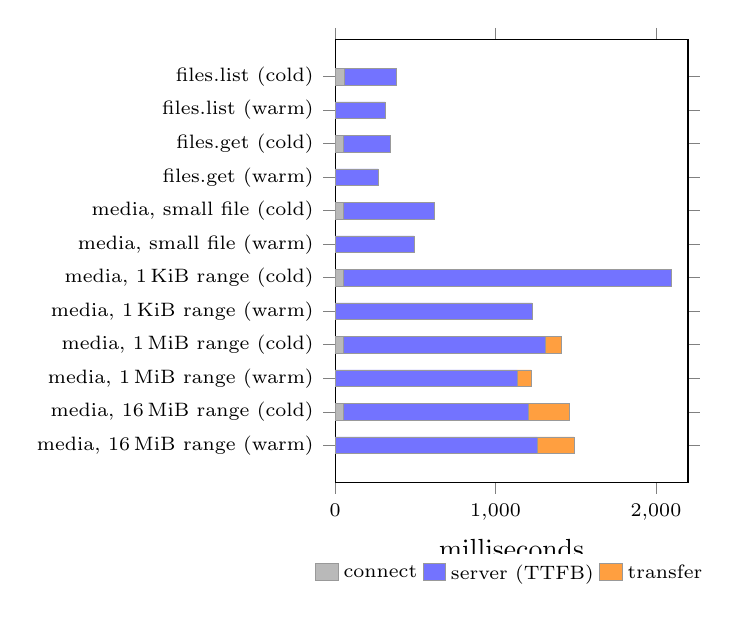
\begin{tikzpicture}
\begin{axis}[
  xbar stacked, width=0.50\columnwidth, height=7.2cm,
  bar width=6pt, xmin=0, xmax=2200,
  scaled x ticks=false, xtick={0,1000,2000},
  xlabel={milliseconds}, xlabel near ticks,
  ytick=data, symbolic y coords={{files.list (cold)}, {files.list (warm)}, {files.get (cold)}, {files.get (warm)}, {media, small file (cold)}, {media, small file (warm)}, {media, 1\,KiB range (cold)}, {media, 1\,KiB range (warm)}, {media, 1\,MiB range (cold)}, {media, 1\,MiB range (warm)}, {media, 16\,MiB range (cold)}, {media, 16\,MiB range (warm)}},
  y dir=reverse, yticklabel style={font=\scriptsize},
  xticklabel style={font=\scriptsize}, tick align=outside,
  legend style={font=\scriptsize, at={(0.5,-0.16)}, anchor=north,
                legend columns=3, draw=none},
  every axis plot/.append style={draw=black!40, line width=0.2pt},
]
\addplot[fill=gray!55] coordinates {(54.3,{files.list (cold)}) (0.0,{files.list (warm)}) (52.4,{files.get (cold)}) (0.0,{files.get (warm)}) (52.9,{media, small file (cold)}) (0.0,{media, small file (warm)}) (53.6,{media, 1\,KiB range (cold)}) (0.0,{media, 1\,KiB range (warm)}) (50.5,{media, 1\,MiB range (cold)}) (0.0,{media, 1\,MiB range (warm)}) (47.5,{media, 16\,MiB range (cold)}) (0.0,{media, 16\,MiB range (warm)})};
\addlegendentry{connect}
\addplot[fill=blue!55] coordinates {(325.3,{files.list (cold)}) (310.9,{files.list (warm)}) (288.9,{files.get (cold)}) (268.0,{files.get (warm)}) (562.5,{media, small file (cold)}) (492.5,{media, small file (warm)}) (2044.8,{media, 1\,KiB range (cold)}) (1226.0,{media, 1\,KiB range (warm)}) (1257.7,{media, 1\,MiB range (cold)}) (1134.7,{media, 1\,MiB range (warm)}) (1157.7,{media, 16\,MiB range (cold)}) (1257.9,{media, 16\,MiB range (warm)})};
\addlegendentry{server (TTFB)}
\addplot[fill=orange!75] coordinates {(0.5,{files.list (cold)}) (0.5,{files.list (warm)}) (0.4,{files.get (cold)}) (0.4,{files.get (warm)}) (0.0,{media, small file (cold)}) (0.0,{media, small file (warm)}) (0.1,{media, 1\,KiB range (cold)}) (0.2,{media, 1\,KiB range (warm)}) (102.2,{media, 1\,MiB range (cold)}) (87.5,{media, 1\,MiB range (warm)}) (253.2,{media, 16\,MiB range (cold)}) (230.8,{media, 16\,MiB range (warm)})};
\addlegendentry{transfer}
\end{axis}
\end{tikzpicture}

\caption{Latency decomposition by request kind, medians of five samples,
measured with raw sockets so each phase is timed separately
(\texttt{helpers.latency\_breakdown}). Each shape appears twice: \emph{cold}
pays connection setup, \emph{warm} reuses an established connection, which is
what the extension's per-thread client does after its first call. The
\texttt{send} phase is 0.0\,ms everywhere and is merged into
\emph{connect}. \textbf{Server time to first byte is essentially the whole
cost at every shape.}}
\label{fig:breakdown}
\end{figure}

The result is stark. At every request shape, the dominant segment is the
server's time to first byte, and it is not close. A 1\,KiB ranged read of the
87\,MB object spends 1226\,ms waiting for Google's first byte and 0.2\,ms
receiving the body. Connection setup --- DNS, TCP and TLS together --- is 48--54\,ms
cold and zero warm. Body transfer only becomes visible at 16\,MiB, where
231\,ms moves the bytes at roughly 70\,MB/s.

\textbf{This corrects a claim we made from indirect evidence.} Replacing a
fresh TLS client per request with a reused per-thread connection had moved the
median request from 1558\,ms to 1334\,ms, and we had attributed that 224\,ms to
connection establishment. Measured directly, the handshake is 33--35\,ms and
the whole of setup is at most 54\,ms. The reuse experiment was a real
improvement, but it cannot have been paying for what we said it was; the
remainder is a difference between the two client configurations we did not
isolate. The direct decomposition supersedes the inference.

\textbf{What the decomposition means.} The residual is Google's service time,
not transfer, and that closes off an entire class of client-side work.
No amount of connection pooling, pipelining or buffer tuning can move a number
that is spent inside somebody else's service before the first byte leaves it.
The only remaining lever is issuing fewer requests, which is precisely what the
block cache does --- and it also explains why the cache's benefit saturates
(Table~\ref{tab:blocksweep}) rather than scaling with the reduction in request
count. It further explains the shape anomaly of
Section~\ref{sec:background}: a 1\,KiB and a 1\,MiB range cost the same because
neither is paying for bytes.

\begin{figure*}[t]
\centering
% GENERATED by e2e/helpers/plot_timeline.py -- do not edit by hand.
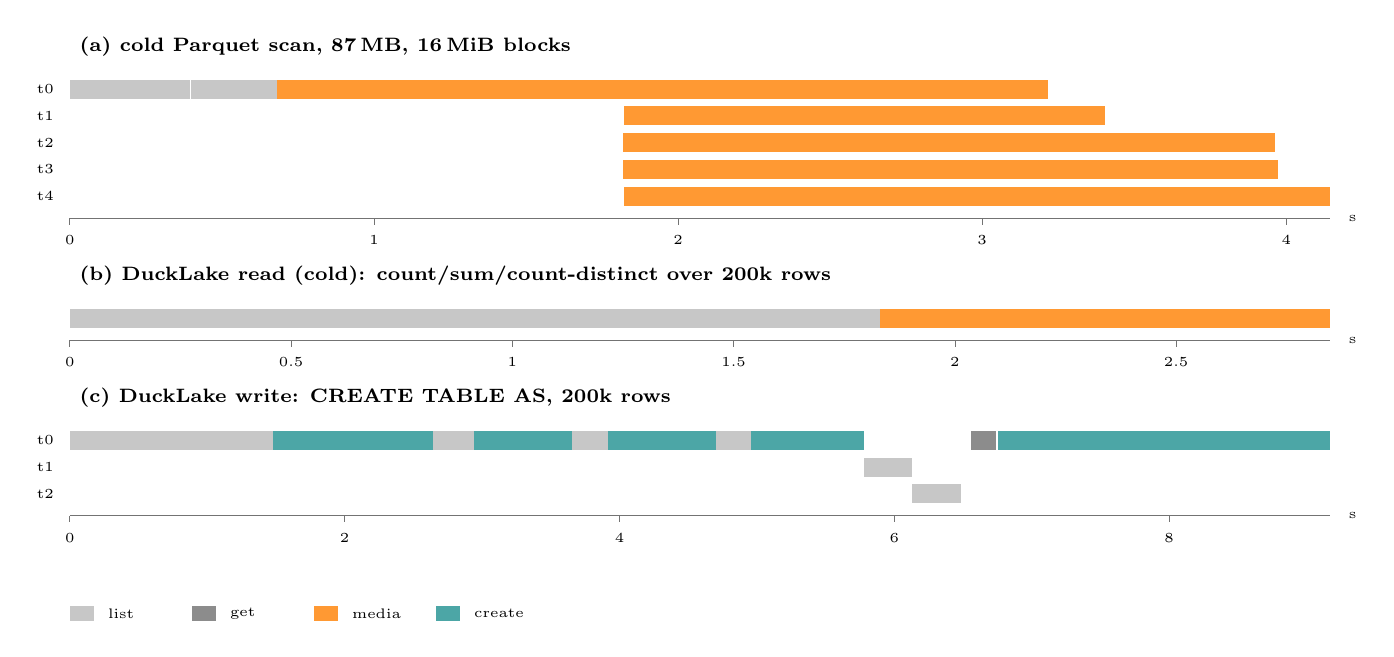
\begin{tikzpicture}[x=1cm, y=1cm]
% --- (a) cold Parquet scan, 87\,MB, 16\,MiB blocks ---
\node[anchor=west, font=\scriptsize\bfseries] at (0,0.42) {(a) cold Parquet scan, 87\,MB, 16\,MiB blocks};
\fill[black!22] (0.000,0.000) rectangle (1.531,-0.240);
\fill[black!22] (1.532,0.000) rectangle (2.632,-0.240);
\fill[orange!80] (2.633,0.000) rectangle (7.024,-0.240);
\fill[orange!80] (7.028,0.000) rectangle (12.428,-0.240);
\fill[orange!80] (7.031,-0.340) rectangle (13.151,-0.580);
\fill[orange!80] (7.029,-0.680) rectangle (15.300,-0.920);
\fill[orange!80] (7.030,-1.020) rectangle (15.344,-1.260);
\fill[orange!80] (7.031,-1.360) rectangle (16.000,-1.600);
\node[anchor=east, font=\tiny] at (-0.08,-0.120) {t0};
\node[anchor=east, font=\tiny] at (-0.08,-0.460) {t1};
\node[anchor=east, font=\tiny] at (-0.08,-0.800) {t2};
\node[anchor=east, font=\tiny] at (-0.08,-1.140) {t3};
\node[anchor=east, font=\tiny] at (-0.08,-1.480) {t4};
\draw[black!55, line width=0.3pt] (0,-1.760) -- (16.00,-1.760);
\draw[black!55, line width=0.3pt] (0.000,-1.760) -- (0.000,-1.840);
\node[anchor=north, font=\tiny] at (0.000,-1.860) {0};
\draw[black!55, line width=0.3pt] (3.862,-1.760) -- (3.862,-1.840);
\node[anchor=north, font=\tiny] at (3.862,-1.860) {1};
\draw[black!55, line width=0.3pt] (7.724,-1.760) -- (7.724,-1.840);
\node[anchor=north, font=\tiny] at (7.724,-1.860) {2};
\draw[black!55, line width=0.3pt] (11.586,-1.760) -- (11.586,-1.840);
\node[anchor=north, font=\tiny] at (11.586,-1.860) {3};
\draw[black!55, line width=0.3pt] (15.449,-1.760) -- (15.449,-1.840);
\node[anchor=north, font=\tiny] at (15.449,-1.860) {4};
\node[anchor=west, font=\tiny] at (16.12,-1.760) {s};
% --- (b) DuckLake read (cold): count/sum/count-distinct over 200k rows ---
\node[anchor=west, font=\scriptsize\bfseries] at (0,-2.49) {(b) DuckLake read (cold): count/sum/count-distinct over 200k rows};
\fill[black!22] (0.000,-2.910) rectangle (1.926,-3.150);
\fill[black!22] (1.927,-2.910) rectangle (4.213,-3.150);
\fill[black!22] (4.213,-2.910) rectangle (5.739,-3.150);
\fill[black!22] (5.739,-2.910) rectangle (7.203,-3.150);
\fill[black!22] (7.203,-2.910) rectangle (8.854,-3.150);
\fill[black!22] (8.854,-2.910) rectangle (10.293,-3.150);
\fill[orange!80] (10.294,-2.910) rectangle (16.000,-3.150);
\draw[black!55, line width=0.3pt] (0,-3.310) -- (16.00,-3.310);
\draw[black!55, line width=0.3pt] (0.000,-3.310) -- (0.000,-3.390);
\node[anchor=north, font=\tiny] at (0.000,-3.410) {0};
\draw[black!55, line width=0.3pt] (2.810,-3.310) -- (2.810,-3.390);
\node[anchor=north, font=\tiny] at (2.810,-3.410) {0.5};
\draw[black!55, line width=0.3pt] (5.620,-3.310) -- (5.620,-3.390);
\node[anchor=north, font=\tiny] at (5.620,-3.410) {1};
\draw[black!55, line width=0.3pt] (8.430,-3.310) -- (8.430,-3.390);
\node[anchor=north, font=\tiny] at (8.430,-3.410) {1.5};
\draw[black!55, line width=0.3pt] (11.240,-3.310) -- (11.240,-3.390);
\node[anchor=north, font=\tiny] at (11.240,-3.410) {2};
\draw[black!55, line width=0.3pt] (14.050,-3.310) -- (14.050,-3.390);
\node[anchor=north, font=\tiny] at (14.050,-3.410) {2.5};
\node[anchor=west, font=\tiny] at (16.12,-3.310) {s};
% --- (c) DuckLake write: CREATE TABLE AS, 200k rows ---
\node[anchor=west, font=\scriptsize\bfseries] at (0,-4.04) {(c) DuckLake write: CREATE TABLE AS, 200k rows};
\fill[black!22] (0.000,-4.460) rectangle (0.707,-4.700);
\fill[black!22] (0.707,-4.460) rectangle (1.182,-4.700);
\fill[black!22] (1.182,-4.460) rectangle (1.658,-4.700);
\fill[black!22] (1.658,-4.460) rectangle (2.140,-4.700);
\fill[black!22] (2.140,-4.460) rectangle (2.577,-4.700);
\fill[teal!70] (2.578,-4.460) rectangle (4.606,-4.700);
\fill[black!22] (4.606,-4.460) rectangle (5.126,-4.700);
\fill[teal!70] (5.126,-4.460) rectangle (6.378,-4.700);
\fill[black!22] (6.378,-4.460) rectangle (6.840,-4.700);
\fill[teal!70] (6.840,-4.460) rectangle (8.210,-4.700);
\fill[black!22] (8.210,-4.460) rectangle (8.655,-4.700);
\fill[teal!70] (8.655,-4.460) rectangle (10.081,-4.700);
\fill[black!22] (10.081,-4.800) rectangle (10.689,-5.040);
\fill[black!22] (10.691,-5.140) rectangle (11.314,-5.380);
\fill[black!45] (11.449,-4.460) rectangle (11.766,-4.700);
\fill[teal!70] (11.782,-4.460) rectangle (16.000,-4.700);
\node[anchor=east, font=\tiny] at (-0.08,-4.580) {t0};
\node[anchor=east, font=\tiny] at (-0.08,-4.920) {t1};
\node[anchor=east, font=\tiny] at (-0.08,-5.260) {t2};
\draw[black!55, line width=0.3pt] (0,-5.540) -- (16.00,-5.540);
\draw[black!55, line width=0.3pt] (0.000,-5.540) -- (0.000,-5.620);
\node[anchor=north, font=\tiny] at (0.000,-5.640) {0};
\draw[black!55, line width=0.3pt] (3.490,-5.540) -- (3.490,-5.620);
\node[anchor=north, font=\tiny] at (3.490,-5.640) {2};
\draw[black!55, line width=0.3pt] (6.980,-5.540) -- (6.980,-5.620);
\node[anchor=north, font=\tiny] at (6.980,-5.640) {4};
\draw[black!55, line width=0.3pt] (10.470,-5.540) -- (10.470,-5.620);
\node[anchor=north, font=\tiny] at (10.470,-5.640) {6};
\draw[black!55, line width=0.3pt] (13.960,-5.540) -- (13.960,-5.620);
\node[anchor=north, font=\tiny] at (13.960,-5.640) {8};
\node[anchor=west, font=\tiny] at (16.12,-5.540) {s};
\fill[black!22] (0.00,-6.69) rectangle (0.30,-6.87);
\node[anchor=west, font=\tiny] at (0.36,-6.78) {list};
\fill[black!45] (1.55,-6.69) rectangle (1.85,-6.87);
\node[anchor=west, font=\tiny] at (1.91,-6.78) {get};
\fill[orange!80] (3.10,-6.69) rectangle (3.40,-6.87);
\node[anchor=west, font=\tiny] at (3.46,-6.78) {media};
\fill[teal!70] (4.65,-6.69) rectangle (4.95,-6.87);
\node[anchor=west, font=\tiny] at (5.01,-6.78) {create};
\end{tikzpicture}

\caption{Every Drive API call of three workloads, on a wall-clock axis. Rows
are DuckDB threads; each bar is one call, coloured by kind. Captured with
\texttt{GDRIVE\_TRACE\_FILE} (Section~\ref{sec:tracing}); the axes are
independent because the runs differ by 3$\times$ in length. Metadata calls are
deliberately muted, so a panel that is mostly grey is a panel that mostly is
not moving data --- which is what (b) and (c) are.}
\label{fig:flame}
\end{figure*}

\textbf{From cost to critical path.}
Figure~\ref{fig:flame} is the same data arranged by time rather than by
request. The distinction matters more here than it would against an object
store: with a per-request floor above one second and eighteen concurrent
handles, total runtime is governed by which requests overlap rather than by
what each costs. The overlap view is what killed the read-ahead buffer of
Section~\ref{sec:blockcache}: a per-handle optimisation cannot see locality
spread across handles. Table~\ref{tab:latency} cannot answer that question.

\textbf{A scan is a serial prologue followed by a parallel scan.}
Panel (a) splits cleanly in two. For the first 3.0\,s --- 48\% of a 6.2\,s query
--- exactly one thread is doing anything: two \texttt{files.list} calls to
resolve the path, one \texttt{files.get} for metadata, then a single 2.0\,s
media request for the Parquet footer. Only then do five threads start fetching
16\,MiB blocks concurrently, finishing in 3.2\,s of wall-clock against 10.3\,s
of summed request time. The parallel half behaves exactly as the block cache
intends. The serial half is untouched by any amount of block tuning, which
explains why Table~\ref{tab:blocksweep}'s block-size sweep produces such small
differences: it is optimising the half of the query that was already fast.

\textbf{A DuckLake read is mostly path resolution.}
Panel (b) is more extreme. Of 3.2\,s, six sequential \texttt{files.list} calls
consume the first 1.7\,s, a \texttt{files.get} takes another 0.2\,s, and a
single 1.0\,s media request moves the only bytes in the query. \textbf{62\% of
a cold DuckLake read is spent discovering where the data is}, on one thread,
before any of it is requested. Drive's missing path addressing (R-1) appears
here as a critical path, not just a request count. This is the strongest
available argument for the \texttt{gdrive://id:} form and for keeping
DuckLake's data path shallow.

\textbf{A DuckLake write is mostly scaffolding.}
Panel (c) is entirely serial --- one thread, 9.7\,s, sixteen calls --- and
alternates \texttt{files.list} with \texttt{files.create} in a way that makes
the cause obvious: the writer is creating the data path one directory segment
at a time, listing each parent first to see whether it already exists. Five
listings and four creates, about 5.2\,s, elapse before the data file itself is
written by the final 2.6\,s \texttt{files.create}. \textbf{Roughly three
quarters of the write is directory scaffolding.} It is also one-off per data
path rather than per row, which is why the effect would be invisible in a
throughput number and why the recommendation it produces --- create the
directory tree once, then write into it --- is not the one a bandwidth
measurement would suggest.

Taken together the three panels answer the question
Section~\ref{sec:ducklake}'s totals cannot: on Drive, a lakehouse workload is
dominated by \emph{metadata serialisation}, not by transfer. That is a
different problem from the one the block cache solves, and it is where the
remaining headroom is. Section~\ref{sec:evalrefresh} takes the first bite out
of it; the panels shown here are post-optimisation, and the \texttt{files.get}
that used to sit between the listings and the first media request in (a) and
(b) is already gone.

\subsection{Eliminating the Redundant Metadata Refresh}
\label{sec:evalrefresh}

Figure~\ref{fig:flame} did not only describe the system; it changed it. The
grey serial runs in panels (b) and (c) prompted the two skips of
Section~\ref{sec:skiprefresh}, and Table~\ref{tab:refresh} measures what they
bought. The workload is a read across 150 CSV files under one prefix --- a
deliberately metadata-heavy shape, and the shape a lakehouse snapshot actually
has.

\begin{table}[t]
\caption{Read across 150 files, cold process, three repeats, reported by
minimum. \texttt{files.get} column counts per-open metadata refreshes; the
second row additionally takes \texttt{files.list} from 151 to 3. Each A/B is
the same binary with one change disabled, so nothing else varies.}
\label{tab:refresh}
\small
\begin{tabular}{lrr}
\toprule
& \texttt{files.get} & wall-clock \\
\midrule
Before                                   & 150 & 17.32\,s \\
Skip the redundant refresh               & 0 & 13.51\,s \\
\quad + cache the glob's own listing     & \textbf{0} & \textbf{9.25\,s} \\
\bottomrule
\end{tabular}
\end{table}

A second change, found by tracing the same workload, removed the other half.
\texttt{Glob} listed a directory, matched locally, returned, and \emph{discarded
the listing} --- so DuckDB's multi-file reader then re-resolved each of the 150
leaves individually. Caching what the glob already held takes 151 listings to
3. Table~\ref{tab:refresh} reports both.

The call count is exact and deterministic: 150 metadata requests become none.
The wall-clock saving, 22\%, is smaller than $150 \times 268$\,ms because
DuckDB opens files in parallel, so most of those requests were overlapping
rather than serialised. Figure~\ref{fig:breakdown}'s per-request costs cannot
be multiplied by a count to predict a total; that mistake produced this
paper's original round-trip estimate. The call count matters in its own right:
Drive enforces per-user API quotas that object stores do not, so a query that
costs 150 fewer requests is faster and cheaper against a limit users actually
hit.

Two effects that this table does not show. First, on a single-file cold scan
the saving is one request, and it disappears into run-to-run variance; the
optimisation matters in proportion to file count, which is why we measure it at
150. Second, our own headline benchmark could not have detected any of this ---
it addresses the fixture as \texttt{gdrive://id:}, the form that skips
resolution entirely and so never had a redundant refresh to remove. A
regression here would have been invisible to the only performance test we run
in CI.

\subsection{Cold Single-File Scan}

\begin{table}[t]
\caption{Cold scan of the same 87\,MB Parquet file (byte-identical in every
backend), three columns aggregated, nine repeats. \textbf{The two sessions are
reported separately and ratios never cross them}, because the object-store
denominator moves more between sessions than the effects being measured.}
\label{tab:coldscan}
\small
\begin{tabular}{lrrr}
\toprule
Backend & min & median & vs.\ object store \\
\midrule
\multicolumn{4}{l}{\emph{Session A --- GCS denominator}} \\
Local disk                          & 0.12\,s & 0.13\,s & 0.09$\times$ \\
\texttt{gs://} (europe-west3)       & 1.34\,s & 1.65\,s & 1.00$\times$ \\
\texttt{gdrive://}, defaults        & 4.09\,s & 4.67\,s & \textbf{3.05$\times$} \\
\texttt{gdrive://}, 128\,MiB blocks & 2.70\,s & 2.93\,s & \textbf{2.02$\times$} \\
\addlinespace
\multicolumn{4}{l}{\emph{Session B --- S3 denominator}} \\
Local disk                          & 0.13\,s & 0.14\,s & 0.12$\times$ \\
\texttt{s3://} (eu-central-1)       & 1.11\,s & 1.24\,s & 1.00$\times$ \\
\texttt{gdrive://}, defaults        & 3.86\,s & 4.48\,s & \textbf{3.48$\times$} \\
\texttt{gdrive://}, 128\,MiB blocks & 2.58\,s & 2.75\,s & \textbf{2.32$\times$} \\
\addlinespace
Download, then query locally        & \todonum{} & \todonum{} & \todonum{} \\
\bottomrule
\end{tabular}
\end{table}

Table~\ref{tab:coldscan} gives the headline result: roughly 3$\times$ object
storage at the defaults, 2$\times$ tuned, against roughly 30$\times$ for a local
file. We set ourselves a 3$\times$ gate before measuring, and against GCS the
default configuration sits \emph{on} it --- 3.05$\times$ on minima, 2.83$\times$
on medians. Calling that a clean pass or a clean fail would both overstate what
was measured.

\textbf{The denominator is the least stable number in the table.} Against S3 in
Frankfurt the same extension, on the same file, measures 3.48$\times$ rather
than 3.05$\times$ --- not because anything got slower, but because S3 answered
in 1.11\,s where GCS took 1.34\,s. The Drive numbers agree closely across the
two sessions (3.86 vs 4.09\,s, within the 9\% run-to-run spread we see on that
leg); the object stores do not. This is the same effect that made an earlier
three-repeat protocol report PASS once and FAIL three times on identical code,
so we report two labelled sessions rather than one merged table with a single
ratio. A paper that quoted ``2$\times$ object storage'' by pairing the best
Drive run with the slowest denominator would not be wrong about any individual
measurement, and would still be misleading.

\subsection{Block-Size Sensitivity}

Two properties of the block cache behave differently and must be measured
separately. Request count is deterministic, so a single run establishes it
exactly (Table~\ref{tab:blockreqs}). Wall-clock time is not, and an early
two-sample sweep led us to a conclusion that five samples reversed.

\begin{table}[t]
\caption{Media requests issued by one scan, by
\texttt{gdrive\_block\_size\_bytes}. Deterministic, so one run suffices.}
\label{tab:blockreqs}
\footnotesize
\setlength{\tabcolsep}{4pt}
\begin{tabular}{lrrrrrr}
\toprule
Block size & 0 & 4\,MiB & 8\,MiB & 16\,MiB & 32\,MiB & 128\,MiB \\
\midrule
Media requests & 35 & 21 & 11 & 6 & 3 & 1 \\
\bottomrule
\end{tabular}
\end{table}

\begin{table}[t]
\caption{Block size against wall-clock, five samples per cell. The footer-only
column is the counterweight the first sweep omitted. Times include process
start-up and \texttt{CREATE SECRET}; the comparison between rows is what
matters.}
\label{tab:blocksweep}
\small
\begin{tabular}{lrrrr}
\toprule
& \multicolumn{2}{c}{full scan} & \multicolumn{2}{c}{\texttt{count(*)}} \\
\cmidrule(lr){2-3}\cmidrule(lr){4-5}
Block size & min & median & min & median \\
\midrule
16\,MiB (default) & 5.01\,s & \textbf{5.43\,s} & 2.31\,s & \textbf{2.61\,s} \\
32\,MiB           & 4.75\,s & 5.47\,s & 2.81\,s & 2.85\,s \\
64\,MiB           & 4.69\,s & 5.05\,s & 2.73\,s & 2.82\,s \\
128\,MiB          & \textbf{3.34\,s} & \textbf{3.49\,s} & 3.23\,s & \textbf{3.40\,s} \\
\bottomrule
\end{tabular}
\end{table}

Three findings were not clear in advance. First, \textbf{fewer requests help
far less than the per-request floor predicts}. Collapsing 35 requests to
one removes about a second, not thirty, because the 35 were already spread
across 18 threads --- the floor was being paid roughly twice in sequence, not
thirty-five times. Second, \textbf{4\,MiB is worse than no cache at all}: small
blocks add bytes without removing enough requests, so the curve is not
monotonic and guessing a block size without measuring would have made the
system slower. Third, \textbf{32\,MiB was noise}. At two samples it looked like
a free 0.08\,s improvement over the default; at five its median is worse and
its footer cost is 0.24\,s higher. We came close to changing a default on the
strength of two samples of a workload whose median moves by 400\,ms between
runs.

We keep 16\,MiB as the default. 128\,MiB buys about 1.9\,s on a full scan and
costs about 0.8\,s on a footer query, and only two such blocks fit inside the
256\,MiB cache cap, so a multi-file scan would thrash. Users whose workload is
large sequential scans should set it explicitly and use the
\texttt{gdrive://id:} form, which is the fastest configuration we measured;
that combination is documented rather than defaulted.

\subsection{DuckLake End to End}
\label{sec:ducklake}

\begin{table}[t]
\caption{DuckLake with its \texttt{DATA\_PATH} on each backend and its catalog
local in all three. Wall-clock and storage API calls per operation.}
\label{tab:ducklake}
\small
\begin{tabular}{lrrrrrr}
\toprule
& \multicolumn{2}{c}{\texttt{s3://}} & \multicolumn{2}{c}{\texttt{gs://}} & \multicolumn{2}{c}{\texttt{gdrive://}} \\
\cmidrule(lr){2-3}\cmidrule(lr){4-5}\cmidrule(lr){6-7}
Operation & s & calls & s & calls & s & calls \\
\midrule
\texttt{CREATE TABLE AS}  & \todonum{} & \todonum{} & \todonum{} & \todonum{} & \todonum{} & \todonum{} \\
\texttt{INSERT} (append)  & \todonum{} & \todonum{} & \todonum{} & \todonum{} & \todonum{} & \todonum{} \\
\texttt{DELETE}           & \todonum{} & \todonum{} & \todonum{} & \todonum{} & \todonum{} & \todonum{} \\
Scan, cold                & \todonum{} & \todonum{} & \todonum{} & \todonum{} & \todonum{} & \todonum{} \\
Time-travel read          & \todonum{} & \todonum{} & \todonum{} & \todonum{} & \todonum{} & \todonum{} \\
Compaction                & \todonum{} & \todonum{} & \todonum{} & \todonum{} & \todonum{} & \todonum{} \\
\bottomrule
\end{tabular}
\end{table}

Table~\ref{tab:ducklake} is the experiment the rest of the paper exists to
support. The workload is the one already encoded in our live suite: create a
table of 20\,000 rows, append 5\,000, delete a seventh of them, read the
pre-append snapshot by version, and compact. The catalog is a local DuckDB file
in all three configurations; only the data path moves. That is the supported
shape, and it is the shape Section~\ref{sec:thesis} argues for.

Reporting API calls alongside wall-clock is what makes the table diagnostic
rather than merely comparative. Where Drive is slower, the count says whether
the cause is per-request latency or a request pattern we could improve.

\subsection{The Effect of DuckLake's Local Cache}

DuckLake caches immutable data files locally. Because Drive's per-request floor
is three orders of magnitude above an object store's, we expect that cache to
be worth disproportionately more on Drive than on S3 or GCS ---
Table~\ref{tab:dlcache} tests it. The quantity of interest is not the speed-up
on each backend but the \emph{ratio of speed-ups}: if caching narrows the
Drive-versus-S3 gap by more than it narrows any other gap, then the practical
advice for a Drive-backed lakehouse is different from the advice for an
object-store-backed one, and that is the most directly actionable result this
paper can produce.

\begin{table}[t]
\caption{DuckLake scan with its local file cache disabled and enabled.}
\label{tab:dlcache}
\small
\begin{tabular}{lrrr}
\toprule
Backend & cache off & cache on & speed-up \\
\midrule
\texttt{s3://}     & \todonum{} & \todonum{} & \todonum{} \\
\texttt{gs://}     & \todonum{} & \todonum{} & \todonum{} \\
\texttt{gdrive://} & \todonum{} & \todonum{} & \todonum{} \\
\bottomrule
\end{tabular}
\end{table}

The exact option names governing this cache are pinned to the DuckLake version
under test and are enumerated from \texttt{duckdb\_settings()} rather than
quoted from documentation, since the caching surface has changed between
releases and a separate disk-cache extension exists that must not be conflated
with it. \todonum{pin the DuckLake version and its cache settings}

\subsection{Write Path and Concurrency}

Table~\ref{tab:writes} covers upload throughput against size, the cost of
creating a folder, and DuckLake commit latency; Figure~\ref{fig:threads} covers
scaling. The property to check in the latter is not that time falls with
threads --- it will, since decompression is the parallel part --- but that
request count stays \emph{flat}. A rising count would mean the single-flight
caches of Section~\ref{sec:resolution} are leaking, which is precisely the
regression that produced 19 metadata calls for one query before those caches
existed.

\begin{table}[t]
\caption{Write path.}
\label{tab:writes}
\small
\begin{tabular}{lrr}
\toprule
Operation & time & effective MB/s \\
\midrule
Upload 1\,MiB           & \todonum{} & \todonum{} \\
Upload 16\,MiB          & \todonum{} & \todonum{} \\
Upload 128\,MiB         & \todonum{} & \todonum{} \\
Create one folder       & \todonum{} & --- \\
DuckLake commit (append)& \todonum{} & --- \\
\bottomrule
\end{tabular}
\end{table}

\begin{figure}[t]
\centering
\fbox{\parbox[c][3.6cm][c]{0.92\columnwidth}{\centering
\todonum{Figure~\ref{fig:threads}: scan wall-clock and total Drive API calls
against \texttt{SET threads} $\in \{1,4,8,16,32\}$, two y-axes. Produced by
\texttt{bench.py --threads-sweep}, reading \texttt{gdrive\_stats()}.}}}
\caption{Thread scaling. Time should fall; request count should not rise.}
\label{fig:threads}
\end{figure}

\subsection{A Negative Result}

The natural first optimisation for high per-request latency is to coalesce
adjacent ranges, and an external review of Drive read performance recommended
exactly that, on a 10--16\,MB threshold, predicting it would ``easily bridge the
performance gap''. It does not, and the reason is visible only in a trace. The
benchmark query issues 35 ranged GETs covering 54.9\,MB of the 87\,MB file;
sorted by offset, the gaps alternate between 1929\,KB and zero, so half of all
requests begin exactly where another ends. Those 35 reads are spread across 18
file handles, and \emph{no} adjacent pair shares a handle. A per-handle
read-ahead buffer therefore cannot see the adjacency at all. We implemented it
and measured: request count unchanged, bytes transferred inflated from
54.9\,MB to 136\,MB. It was reverted, and the cache became file-level instead.

We report this at length because the recommendation was reasonable, the
reasoning behind it was correct as far as it went, and the only thing that
distinguished it from the right answer was a trace showing which handle each
request belonged to. It is also the clearest argument for
Figure~\ref{fig:flame}.

%% =====================================================================
\section{When You Should Not Use This}
\label{sec:notthis}
%% OUTLINE (plan sec. 6). Three named alternatives with the trade for each:
%% Drive for desktop on a workstation; rclone mount (the trade is operational,
%% not technical); copy-to-object-storage for a large hot dataset. State that
%% we declined to benchmark the FUSE alternative, and why.

The measurements above bound what this system is good for, and the boundary is
narrower than the engineering might suggest. Three cases are better served by
something else.

\textbf{On a workstation, use the desktop client.} Google Drive for desktop
presents Drive as ordinary local paths. It is faster, needs no extension, and
is correct. This work exists for headless servers, where a logged-in desktop
client is not an option.

\textbf{If a FUSE mount already works, keep it.} \texttt{rclone mount} presents
Drive as a local path and needs no DuckDB extension at all. The trade is
operational rather than technical: a mount to provision and monitor on every
host, and behaviour under concurrency and partial reads that is outside the
query engine's control, against an extension that needs nothing on the host but
itself. We did not benchmark the FUSE alternative. That was a deliberate
scoping decision and it leaves the strongest competing approach formally
unmeasured --- we state the trade rather than claim to have settled it.

\textbf{For a large, hot dataset, copy it to object storage.} A ranged read
from Drive costs 1.2--2.1\,s regardless of how few bytes it requests, against
milliseconds for S3 or GCS, and Drive enforces per-user API quotas that object
storage does not. This is the right tool when Drive is the \emph{system of
record} and the goal is to stop maintaining a second copy --- not when the goal
is a fast warehouse.

The honest summary is that this work buys freshness and the elimination of a
copy, and pays two to three and a half times the query latency of object
storage for it --- plus, for a lakehouse, a metadata prologue that is a larger
share of a small query than the transfer is
(Figure~\ref{fig:flame}).

%% =====================================================================
\section{Related Work and Summary}
\label{sec:related}
%% OUTLINE (plan sec. 7). Comparative, not a survey: DuckDB-Wasm's paged web
%% filesystem (same problem shape, different constraints), httpfs/S3,
%% duckdb-gcs, gsheets, rclone/FUSE, lakehouse formats. Close on the two
%% limitations that would most change the result: resumable uploads, and the
%% absence of any revision-pinned read.

\textbf{Related work.}
DuckDB-Wasm~\cite{duckdbwasm} solves the closest problem: it reads remote data
through a browser-agnostic filesystem using HTTP range requests and
exponentially growing read-ahead buffers to limit request count. The problem
shape is the same --- high-latency, range-capable, non-POSIX storage --- and the
divergence in solution is instructive. Exponential read-ahead works there
because the browser issues its requests through one logical reader; it fails
here because DuckDB's parallel scan spreads adjacent ranges across independent
handles, which is why our cache is file-level and revision-keyed rather than
per-handle. DuckDB's own \texttt{httpfs} addresses S3 and compatible stores,
where every guarantee in Table~\ref{tab:guarantees} that Drive lacks is
present and a ranged read costs milliseconds; the design space is genuinely
different rather than merely tuned differently. Extensions exist for Google
Cloud Storage and for Google Sheets; the former targets storage where a
self-signed JWT authenticates successfully, which is precisely the assumption
that fails for Drive as a Workspace API (Section~\ref{sec:auth}), and the
latter addresses a single native format rather than a filesystem. Against
lakehouse formats --- DuckLake, Iceberg, Delta Lake --- this work is
complementary: we supply a storage layer, and Section~\ref{sec:thesis} argues
their immutability discipline is what makes that layer viable.

\textbf{Summary.}
We built a DuckDB filesystem over storage that provides neither path
addressing, nor unique names, nor atomic replace, nor revision-pinned reads,
nor a conditional request to compensate, and whose per-request cost is nearly
independent of request size. The design
that follows inverts the object-store intuition: fetch more in fewer requests,
cache by revision rather than by path, and refuse to emulate the primitives
that are missing. The result reaches 3.05$\times$ GCS at defaults and
2.02$\times$ tuned on a cold columnar scan. More useful than either number is
the structural finding, and it cuts twice. The guarantees Drive fails to
provide are almost exactly the ones a lakehouse format does not use, so a table
format on Drive is not a workaround but the natural fit --- and the same
immutability that makes it correct is directly exploitable for speed, removing
150 metadata round trips and, with the glob-cache fix alongside it, 47\% of
wall-clock from a 150-file read. The
tooling mattered as much as any single optimisation: the span timeline of
Figure~\ref{fig:flame} is what revealed that a lakehouse workload on Drive is
dominated by serialised metadata rather than transfer, which was invisible in
every aggregate we had measured before building it.

Two limitations would most change this result. Uploads are simple rather than
resumable, so a failed write may or may not have been applied --- the single
largest correctness gap, and the first item of future work. And no read can be
pinned to a revision, so a scan concurrent with an overwrite may mix two of
them; this one we can only report, since Drive exposes no mechanism that would
let us fix it.

\balance
\bibliographystyle{ACM-Reference-Format}
\bibliography{refs}

\end{document}
